\TOWRITE{ALL}{Proofread 1.2 up to 1.2.10}

\TOWRITE{ALL}{Write missing sections 1.2.13 to 1.2.16}

\TOWRITE{Min/Hans}{Mention KPIs somewhere?}

\TODO{Provide contents for empty subsections at the end of section 1.}

\subsection{Methodology}\label{sec:concept_methodology}
\eucommentary{5-8 pages}





% \subsubsection{Concept}%\label{sec:concept}
%
% Open Science is the principle that science, in order to be most
% {impactful} and {socially responsible}, should be done
% {publicly}, with as much of the scientific process and products
% accessible, reviewable, reproducible and reusable by as many members of
% the global community as possible.
%
% There are exciting opportunities for Open Science for almost all academic fields
% in the modern age of computational science. As more and more research takes the
% form of code and/or data, the opportunity to share, reproduce, and reuse
% scientific work is greater than ever, even enabling new forms of
% {interdisciplinary collaboration}, and interoperable and re-usable results and
% tools.
%
%  Simultaneously, there are obstacles -- both technical and social -- to
% making open science and reproducible science a practical reality. The challenges
% include: If a researcher has code and/or data to publish, how is that best
% done? How do researchers learn {best practices for reproducible science} in
% their field? How do previously disconnected fields benefit from each other's
% work as the same computational challenges are faced again and again by different
% communities? How can scientists be encouraged to make their work reproducible?
%
% These are the questions that guide the \TheProject{} project.

\subsubsection{Supporting Open, Useful, and Reproducible Computational
  Environments}\label{sec:SOURCE}

Our project is titled ``\emph{Supporting Open, Useful, and Reproducible Computational Environments.}'':
\begin{itemize}
\item The work done is this project will be \emph{Supporting} scientists in their
  endavours to make their work more reproducible and re-usable.
\item We believe in the value of \emph{Open} science and \emph{Open} source. The
  best reproducibility and re-usability of scientific results is given through
  complete transparency of the steps taken in the derivation of a result. For
  the computational aspects this means to make all simulation and/or
  post-processing and analysis steps open source. While this may not always be
  possible, we advocate such openness as the best practice for reproducible science.

  All work done, including software, training and documentation materials, will
  be open source and available through an open access license.

  (We note that the collective development of the grant proposal you are reading
  is also done as open source, and can be inspected at
  \url{http://github.com/minrk/horizon-widera-2022} for those interested.)

\item Measures towards better reproducibility have to be \emph{Useful} and
  practical: if a proposed approach or tool burdens the scientist with
  additional work, or requires significant additional skills, it becomes less
  likely to be widely accepted.

  The philosophy we support here is that the proposed (Binder) tools for
  reproducibility are based on existing standards which are already
  adopted by many and can be considered best practice.

\item Within the wide field of reproducibility in science, we focus in this
  project on the improvement of the automatic generation of \emph{Reproducible
    Computational Environments}.
  % It is an essential step for reproducible
  % science to be able to setup the correct
  % software environment, before any attempt can be undertaken to reproduce (and
  % thus repeat) the calculation of a result obtained before.
\end{itemize}

\subsubsection{Outline of concept and methodology}

In the following we explain our concept and the technology on which this
proposed project builds in more detail.
\begin{itemize}
\item Sections \fullref{sec:reproducibility} and
  \fullref{sec:reproducibility-challenges} contextualise the proposed work
  within the wide field of reproducibility.
\item Section \fullref{sec:reproducibility-concept} summarises our concept and
  approach concisely.

\item To prepare the more detailed description of the concept and the content of
  the Work Packages, we use Section \fullref{sec:reproducibility-example} and
  \fullref{sec:terminology} to introduce key terminology together with an
  example for computational reproducibility.

\item Sections \fullref{sec:project-jupyter} and \fullref{seq:project-binder}
  introduce the Jupyter and Binder projects, respectively.

%\item Section \fullref{sec:binder-for-reproducibility} explains the use of
%  Binder tools for reproducible science.
\end{itemize}
  
\noindent The methodology for this project is discussed starting in section
\fullref{sec:methodology}.



%\TODO{Do we need to keep anything from the commented out lines here?}

%
% With so much research being done that wants to be Open and Reproducible,
% how can we make Science
%
% \begin{enumerate}
%     \item as \textbf{easy} as possible to share and reproduce?
%     \item as \textbf{useful} as possible to other researchers and the public?
% \end{enumerate}
%
%
%
%
%
% \noindent Our plan for \textbf{increasing the reproducibility of scientific results} can be summarised as:
%
% \begin{enumerate}
% \item improve and maintain \textbf{common software infrastructure} used for
%   reproducing computational results,
% \item develop the Jupyter ecosystem to improve capabilities to \textbf{better
%   serve Reproducible Open Science},
% \item \textbf{guide, validate, and demonstrate} our developments through
%   collaboration with a wide variety of application domains,
% \item enable students and researchers to perform Reproducible Open Science through
%   \textbf{training and education}, and improving inclusiveness by focusing
%   these on under-served and under-represented communities
% \end{enumerate}

\medskip

\subsubsection{Reproducibility}\label{sec:concept}\label{sec:reproducibility}

Before describing the focus of the work that we propose here, we want to embed
this into the much wider context of reproducibility challenges.

We will exclude the challenges of reproducing \emph{experimental} data. Our
study starts at the point where such experimental data is available in digital
form.

We will focus on the challenge of computational reproducibility: can we carry out
the same data analysis, creation of figures and tables as they are presented in
a paper, at a later stage, and get to the same results?

Such tables and figures in a publication may be computed from the analysis of
some type of raw data which could originate an experiment, another publication,
a data base, post-processing of another data set or from executing computer
simulations.

% Where additional software, such as analysis scripts, input files
% and software for the simulation are needed,

\subsubsection{Challenges of Reproducibility}\label{sec:reproducibility-challenges}

The challenges of such ``computational reproducibility'' include:
\begin{itemize}
\item Do we know the protocol, \emph{i.e.} are the different
  processing steps for that data recorded? This could be the order in which
  analysis scripts need to be executed -- for example to compute intermediate
  results -- which will be turned into a figure in the last step?

We will call this sequence of steps the \emph{workflow}. This workflow could be
archived -- for example -- through a \softwarename{README.txt} file, or scanned
pages of a hand-written laboratory notebook as a pdf file, or as a
machine-executable script (or a Jupyter notebook).

This is particularly challenging where software is used which can only be
controlled via a Graphical User Interface, as it may require manual recording
and description of the different clicks and steps in laboratory logbook.

\item Are all the scripts and configuration files (and more generally all
software) that is needed in this process known and archived?

\item Where software is involved, have we recorded which version of that
software is needed (or was used)? If compilation is required, do we know which
compilers (and which version) and which additional dependencies are required?

\item Are there instructions how to obtain / compile the required dependencies,
and the software itself (in particular where this is about simulation based
science or more complex analysis and interpretation software tools)?

\item Where raw data is required, is this archived, accessible, and sufficiently
documented that the format is understandable?
\end{itemize}


\subsubsection{Reproducibility concept}\label{sec:reproducibility-concept}

We can classify the reproducibility challenges listed above into different categories:

\begin{description}
\item[1. Workflow]: Are the processing commands (and their order)
correctly recorded? Do we know which part of the data set the analysis is meant
to be applied to? This is to a significant degree a question of the organisation
and documentation of the research process.

\item[2. Software environment]: Can we recreate the software environment that is
required to execute these commands?

\item[3. Importance]: Is the researcher convinced that investing effort into making
their work more reproducible is a worthwhile investment? This is a wide topic,
touching on expectations, existing cultures, lack of metrics that acknowledge
reproducibility efforts, and policies.

\item[4. Other]: There are other related topics, for example the challenge of
archival of (large) research data sets, of making the data FAIR, and the (for
some domains important) bit-wise reproducibility.
\end{description}

In this proposal, we start from practices that researchers increasingly adopt,
and which we argue are \emph{good reproducibility practices}. We propose to carry
out additional work to \emph{improve the toolset enabling this practice}.

To deal with the \emph{Workflow} challenges, we recommend to automate the
workflow steps as much as possible. In particular, the use of Jupyter Notebooks
to orchestrate the execution of commands seems effective~\cite{Beg2021}.
The use of the notebook is
perceived by many as an improvement of their research effectiveness because
it supports ``Thinking with Code and Data''~\cite{Granger2021}. A such, the
practice of using Notebooks (which helps improving research effectiveness) has
the very positive side effect of making the work more reproducible. (However, we
note that an important task of this project is to support reproducible science
that does not make use of Jupyter Notebooks.)

To deal with the \emph{Software environment} challenge, we recommend to follow
standard practices to describe software requirements. The \emph{focus of this
project is to extend the capabilities of the \repotodocker{} tool} to be able to
\emph{automatically create software environments} based on such software
requirement descriptions.

We can only partially address the \emph{Importance} challenge as this needs
concerted efforts from many stakeholders (such as employers of researchers,
research funders, publishers). However, we will offer training that advocates
the value of open science and that teaches existing best practice in
effective computational science. The step from following such best practice to
making the work reproducible is -- given the Binder tools we want to develop
further here -- relatively small, or even possible without additional effort.

The \emph{Other} challenges are mostly outside the focus of this work
(although our proposal will also assist in reproducible and FAIR data
publishing, see for example Task \taskref{applications}{data-publishing}).


% \subsubsection{Terminology and repository example}\label{sec:reproducibility-example}

\subsubsection{Reproducibility Example}
\label{sec:reproducibility-example} 

\begin{figure}[htb]\centering
  \includegraphics[width=0.9\textwidth]{use-cases-binder-logbook-solution.png}
  \caption{A typical use case for Binder-based reproducibility using Jupyter notebooks in research.
            Image by Juliette Belin for the OpenDreamKit project, used under
            CC-BY-SA.}\label{fig:use-cases-binder}
\end{figure}

We start with a description of a use-case making use of existing Binder-based
tools for computational reproducibility. Start from this base-line, we can
explain what progress and additional impact we will enable through this project.

Figure~\ref{fig:use-cases-binder} depicts how a scientist can use a Jupyter
notebook and the Binder software to make her research results easily
reproducible and re-usable. In short:
\begin{itemize}
\item Scientist Jane has created a notebook that carries out computations or
  data processing and creates a figure based on those results. For the purpose
  of the introduction of this workflow, we assume that
  Figure~\ref{fig:reproducibility-example-covid} shows this figure.

\item She has made the notebook and raw data available in a public repository
  (for our example at\newline
  \mbox{\url{https://github.com/fangohr/reproducibility-repository-example}}).

\item As she has described what software is needed to execute her notebook (more
  details below), it is possible for all interested scientists (and anybody
  else, including the reviewers of this proposal) to \emph{reproduce} her
  figure:

  To reproduce the figure, one needs to visit the URL\newline
  \mbox{\url{https://mybinder.org/v2/gh/fangohr/reproducibility-repository-example/HEAD?labpath=figure1.ipynb}}
  in a browser, and then wait a minute or so for a dedicated computational
  environment to be created and started. Then select 'Run' -> 'Run all cells'
  from the menu of the interactive Jupyter notebook that will appear in the
  browser.

  At that point, the computational steps that Jane has carried out to create her
  result are repeated, and the results are \emph{reproduced}.
  
\item Because all the computational steps are captured in the Jupyter notebook,
  they can be inspected and interrogated if desired. In particular, the steps
  can be modified and re-executed: this allows very efficient \emph{re-use} of
  the results by other researchers.
\end{itemize}

We provide a more detailed description of the components and steps in this
process in the following sections \ref{sec:terminology} to \ref{sec:mybinder}.

The reproducibility workflow shown in Figure~\ref{fig:use-cases-binder} is
working today, and we provide estimates on the number of current users in
section \ref{sec:mybinder}. The work proposed for this project will build on
this existing technology and (i)~make it more robust and easier to use
(\WPref{reproducibility}), and (ii)~extend the functionality (\WPref{impact}) so
that the existing tools can be used in many more use cases
(\WPref{applications}).

We note in particular that the Binder-enabled workflow for reproducibility has
originally been developed to reproduce results that are created within Jupyter
Notebook (as shown in Figure~\ref{fig:use-cases-binder}). As part of this
project, we will extend the Binder tool functionality, so that reproducible
computational environments can be created and used in studies that do not make
use of Jupyter notebooks.

\begin{figure}
  \centering
  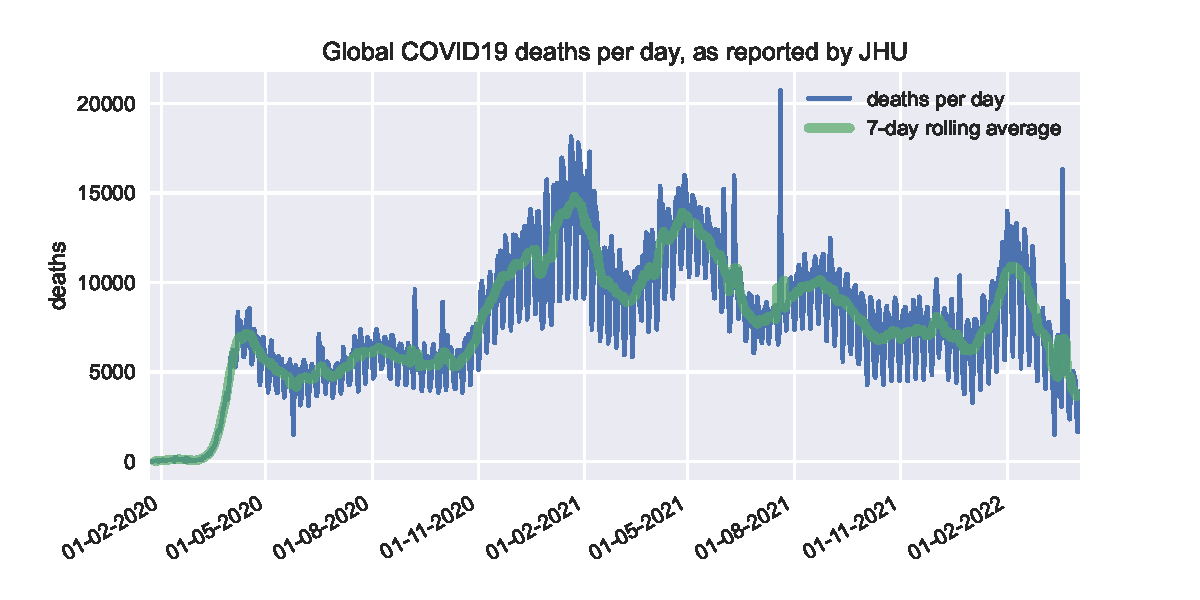
\includegraphics[width=0.8\textwidth]{images/figure1.pdf}
  \caption{Figure (\softwarename{figure1.pdf}) which can be reproduced in our explanatory repository example
    \cite{ReproducibilityRepositoryExample2022}. \label{fig:reproducibility-example-covid}}
\end{figure}


\subsubsection{Terminology}\label{sec:terminology}

For clarity, we define some terms that have been used already above which refer to
throughout this proposal. We illustrate the terms in the context of the
reproducibility example in Section~\ref{sec:reproducibility-example}.

In particular, we imagine that we have a publication that contains
figure~\ref{fig:reproducibility-example-covid} as a result, and we want to
archive and make available \cite{ReproducibilityRepositoryExample2022} the
necessary information for others to reproduce that figure.

\begin{description}
\item[Repository] We refer to a \emph{repository} as a collection of files.

The \emph{purpose} of the repository in our context is to archive information to make
research results reproducible.

Such a repository could be a git repository (which could be hosted on Github,
Bitbucket, Gitlab, or other services), but it could also just be a zip file of a
collection of files.

The repository could be made publicly available, for example through Zenodo,
Figshare, as an electronic supplementary to a publication, or through Github.

It is not unusual that a larger number of files might be
organised in subdirectories within the repository.

Our example repository\footnote{
  https://github.com/fangohr/reproducibility-repository-example/} \cite{ReproducibilityRepositoryExample2022} contains the following files:

\begin{description}
\item[\softwarename{README.md}]: an overview of the content of the repository
\item[\softwarename{figure1.ipynb}]: notebook that creates
  \softwarename{figure1.pdf} from
  the raw data. Could also be realised through a script or other executable
  program of some kind.
\item[\softwarename{requirements.txt}]: software specification
\item[\softwarename{time\_series\_covid19\_deaths\_global.csv}]: raw data
\end{description}

\item[Script] An machine executable file (for example a Bash, Python, Perl
script, Makefile or similar). Such scripts can execute data processing commands,
and are often part of a repository to make the (automatic) reproduction of
results possible.

In our example, the necessary steps to create the figure from the raw data are
gathered in the notebook \texttt{figure1.ipynb}.

\item[Notebook] A Jupyter Notebook. In short, an executable document that can
  combine text, code and computation results. A Jupyter notebook can be used like a
  script. The notebook is explained in Section \fullref{sec:jupyter-notebook}.

\item[Software specification] The software specification depends on the software
  tools used. In our example, the \texttt{requirements.txt} file contains
\begin{verbatim}
pandas==1.3.4
matplotlib==3.4.3
\end{verbatim}
to indicate that we need the pandas and matplotlib package with the respective
versions 1.3.4 and 3.4.3.

\item[Software environment] All the software that needs to be available and
  installed to execute the scripts and (and if desired) Jupyter notebooks.

\item[Project Binder] The Project Binder is described in Section
\ref{seq:project-binder}. It is part of the Jupyter ecosystem of tools, and
allows to convert a repository with Jupyter notebooks into an browser-hosted
environment, in which the notebooks can be executed interactively (and thus
results can be reproduced). 

\item[Binder tools] The Binder tools consist of \binderhub{}
  (Section~\ref{sec:binderhub}) and \repotodocker{} (see
  Section~\ref{sec:repo2docker}) . 

\item[\repotodocker] \repotodocker{} is a tool that can automatically create a
\emph{software environment} (currently within a Docker container) in which the
notebooks and scripts of a repository can be executed 
(Section~\ref{sec:repo2docker} and \ref{binder-how-does-it-work}).
\end{description}

\subsubsection{Project Jupyter}
\label{sec:project-jupyter}

% Figure has been moved into concept.tex. Label remains the same.
% \begin{figure}[htb]\centering
%   \includegraphics[width=0.9\textwidth]{use-cases-binder-logbook-solution.png}
%   \caption{A typical use case for Jupyter notebooks in research.
%             Image by Juliette Belin for the OpenDreamKit project, used under
%             CC-BY-SA.}\label{fig:use-cases-binder}
% \end{figure}

\paragraph{Relationship between the \TheProject{}project and the Jupyter ecosystem}

Some of the team member of the proposed SOURCE project have a track record as
developers and contributors to Project Jupyter and its associated
ecosystem, including Jupyter Notebook.

In opening this section, we'd like to state that the proposed work will improve
the reproducibility of research that uses notebooks, but that it is a key aspect
of the proposal to make the potential impact of the Binder tools for
reproducibility available to those researchers who have no desire or possibility
to use notebooks in their work.

In this section, we introduce key components of project Jupyter to help
contextualise the Binder project that is described subsequently, and the focus
of the proposed work.


% \TheProject has chosen to centre its efforts on the Jupyter software
% ecosystem, in particular Binder and repo2docker.
% Figure~\ref{fig:use-cases-binder} summarises a typical use
% case of Jupyter Notebook and Binder;
% both are described in more detail below.


\paragraph{Project Jupyter}

\emph{Project Jupyter} \cite{Jupyter}, which has grown increasingly popular in the scientific
computing community, has become the \emph{lingua franca} of interactive
computing in both academia and industry \cite{Perkel2018}. The main goal of Project Jupyter
is to provide a consistent set of tools to improve researchers'
workflows from the exploratory phase of the analysis to the communication
of the results \cite{Kluyver2016,Granger2021}.

Split in 2014 from the \emph{IPython Project} \cite{IPython}, Jupyter has grown rapidly in
popularity and adoption both in the industry and academia. We estimate the user
base of the Jupyter notebook to be in the millions \cite{jupyter-grant}. Users range from data
scientists to researchers, educators, and students from many fields,
including journalists and librarians. In 2017, the Jupyter
team was awarded the \emph{ACM Software System Award}, an annual award that
honors people or an organization \emph{"for developing a software system that had a
lasting influence"}. Prior recipients include \emph{Unix}, \emph{TCP/IP}, and
the \emph{World Wide Web} \cite{acm-award}.

A large number of discrete software components make up Project Jupyter.
While these interact with one another, many can be installed separately
to serve various use cases.

% For this proposal, we loosely divide the
% software involved into \emph{Jupyter core} developed under the guidance
% of the developers who started the project, and the broader \emph{Jupyter
% ecosystem} including software developed by third parties,
% which may interact or build upon core Jupyter components.

Some of the components and concepts important to \TheProject are detailed below.

\begin{figure}[ht]\centering
  \centering
  \includegraphics[width=0.9\textwidth]{spectrogram_smaller.png}
  \caption{A notebook document in the Jupyter Notebook interface.}\label{fig:notebook-screenshot}
\end{figure}

\paragraph{Jupyter Notebook}\label{sec:jupyter-notebook} The Jupyter Notebook is
the flagship application of Project Jupyter. 
It allows the creation of notebook documents, containing a mixture of text and
interactively executable code, along with rich output from running that code.
Figure \ref{fig:notebook-screenshot} shows an open notebook including graphs
from an audio processing example. Notebook documents are readily shareable,
providing a popular way to describe and illustrate computational methods and
tools. \TODO{We should update the notebook: (i) point to a github repo with it,
  and (ii) binder-enable it, and (iii) increase the pixel resolution of the
  screen shot. Madison?} \textbf{Jupyter Lab} is the new, modular, extensible
client application for Jupyter notebooks, but the document format, server, and
user model are the same.

\paragraph{JupyterHub}\label{sec:jupyterhub} JupyterHub is a multi-user extension of the Jupyter Notebook.
It runs on one or more notebook servers, for example at a research institution.
Users can log in to author and run notebooks through their web browser, without
needing to install any software on their own computer (because the research
software that is executed is located with the JupyterHub installation at the
research institution).

The communication between the notebook server (for example at the research
institution) and the client (for example the researcher with their laptop in the
home office) is based on the standard https protocol, and the connection is
efficient. The researcher - as the client of the connection to the JupyterHub -
only needs a web browser, and very modest hardware to be able to access
supercomputers or cloud resources remotely.

\TODO{Add an image with a schematic of JupyterHub here?}

Because of these characteristics, many research institutions host their own
JupyterHub service to provide access to large compute and data hosting
hardware~\cite{Fangohr2020}. JupyterHub installations are also seen as important
for EOSC, for example~\cite{panosc-jupyter-binder}. \TODO{Would be good to list
  one or two more EOSC projects / activities / EGI JupyterHub link}


% \medskip\noindent\emph{Jupyter ecosystem}\label{jupyter-ecosystem}
% 
% While Jupyter is a large, distributed, coordinated project,
% the wider community of Jupyter users develops a great deal of
% software with Jupyter integration,
% providing increased or domain-specific functionality,
% building on top of Jupyter, or integrating core Jupyter components in some aspect.
% We call this the \textbf{Jupyter ecosystem}.
% The broader Jupyter ecosystem includes many more projects than we will describe
% here, but a selection of projects which are relevant to
% \TheProject includes:
% 
% \begin{itemize}
%   \item \textbf{Binder} builds on JupyterHub to allow sharing executable
%   environments along with data files and a description of the software components
%   required to run the notebooks. When someone accesses a Binder repository,
%   the service builds the computational environment on demand, allowing them to
%   execute and modify a copy of the notebooks.
%   \textbf{repo2docker} \cite{repo2docker} and \textbf{BinderHub} \cite{binder} are components of the Binder
%   software. \TOWRITE{}{More here, as repo2docker is key}
% \end{itemize}

% \begin{figure}[ht]\centering
%   \includegraphics[width=0.5\textwidth]{ipywidgets_example.png}
%   \caption{An example of using two simple slider widgets to explore the
%   parameter space of a function. The \texttt{@interact} decorator creates
%   the widgets and connects them to the function.}
%   \label{fig:ipywidgets-example}
% \end{figure}

\paragraph{Jupyter notebook and reproducibility}

While Jupyter notebooks can make computational and data-driven research more effective
\cite{Perkel2018,Fangohr2020,Granger2021}, they also have great potential to push
Open and Reproducible Science forward \cite{Beg2021}. The notebook provides a complete
description of a computational and data science study (Step 1 in
figure~\ref{fig:use-cases-binder}), and the notebook can -- in principle -- be
turned into a publication, or can be used to provide the required computation
for a part of a publication, such as a figure (Step 2 in
figure~\ref{fig:use-cases-binder}). Once the researcher has specified what
software is required to execute the notebook (Step 3 in
figure~\ref{fig:use-cases-binder}), the study is completely reproducible by
anyone (Step 4 in figure~\ref{fig:use-cases-binder}).

In this way, the notebook \emph{enables reproducibility} of complex workflows
with minimal additional effort on the user side. This approach is used by a
substantial number of scientists for publications already (for example
\TODO{insert publications with reproducible repositories}): it is hard to prove
but it seems plausible that a significant fraction of the 30,000 sessions
triggered on MyBinder every day are used for reproducible repositories
(Section~\ref{sec:mybinder}).

% HF: this is a reference to the Joel Grus criticism. Not sure if we need it.
% The paper by Beg2021 addresses that in section 9.
(We note in passing that the use of Jupyter notebooks alone does not guarantee
reproducibility: it requires some training and/or experience to be able to specify a
computational environment and to capture in a machine readable way all required
computational steps.)

The Binder tools (Section~\ref{seq:project-binder}) were designed to execute
such notebooks in tailored computational environments which can be created
automatically and on demand (Step 4 in figure~\ref{fig:use-cases-binder}).

This fully-automatic creation of the correct software environment is an
essential aspect of reproducibility that is not widely addressed yet. This
project will address this need, improve the automatic software creation support
for notebook-driven computational research, and make the same improved automatic
software creation support accessible for uses cases without notebooks.

%%% Local Variables:
%%% mode: latex
%%% TeX-master: "proposal"
%%% End:

\subsubsection{Project Binder}\label{seq:project-binder}

The Binder Project \cite{binder} (\url{https://jupyter.org/binder}) is
a subproject of the Jupyter project. The Binder project is formally operating
within the Jupyter ecosystem, but not confined to be useful only for notebooks.

The key components of the Binder software are \repotodocker{}
(Section~\ref{sec:repo2docker}) and \binderhub{}. The \repotodocker{} tool
creates a software environment inside a Docker container from a software
specification in a repository. \binderhub{} starts a Jupyter notebook server
within this container from which the user can execute the notebooks from the
repository.

\emph{\mybinder{}} (see \ref{sec:mybinder}) is a service provided by the \emph{BinderHub
  federation} that collectively host a service running the Binder software
under the URL \url{https://mybinder.org}. This is the service we made use of in
our example in section~\ref{sec:reproducibility-example}.

The focus for this proposal is to improve \repotodocker{}. In particular,
\repotodocker{} solves the software environment challenge (see
Section~\ref{sec:reproducibility-concept}) in a generic way and is independent
from Jupyter notebooks.

\TODO{Add image that depicts this Jupyter/Binder relation ship}.

\paragraph{Basic functionality of Binder}
\label{binder-how-does-it-work}

The currently most common reproducibility use case -- with the current state of the Binder
tools -- is the one we introduced in
Section~\ref{sec:reproducibility-example}. We will use this to
describe the role of the individual components of Binder:


\begin{figure}
  \begin{minipage}[b]{0.67\textwidth}
    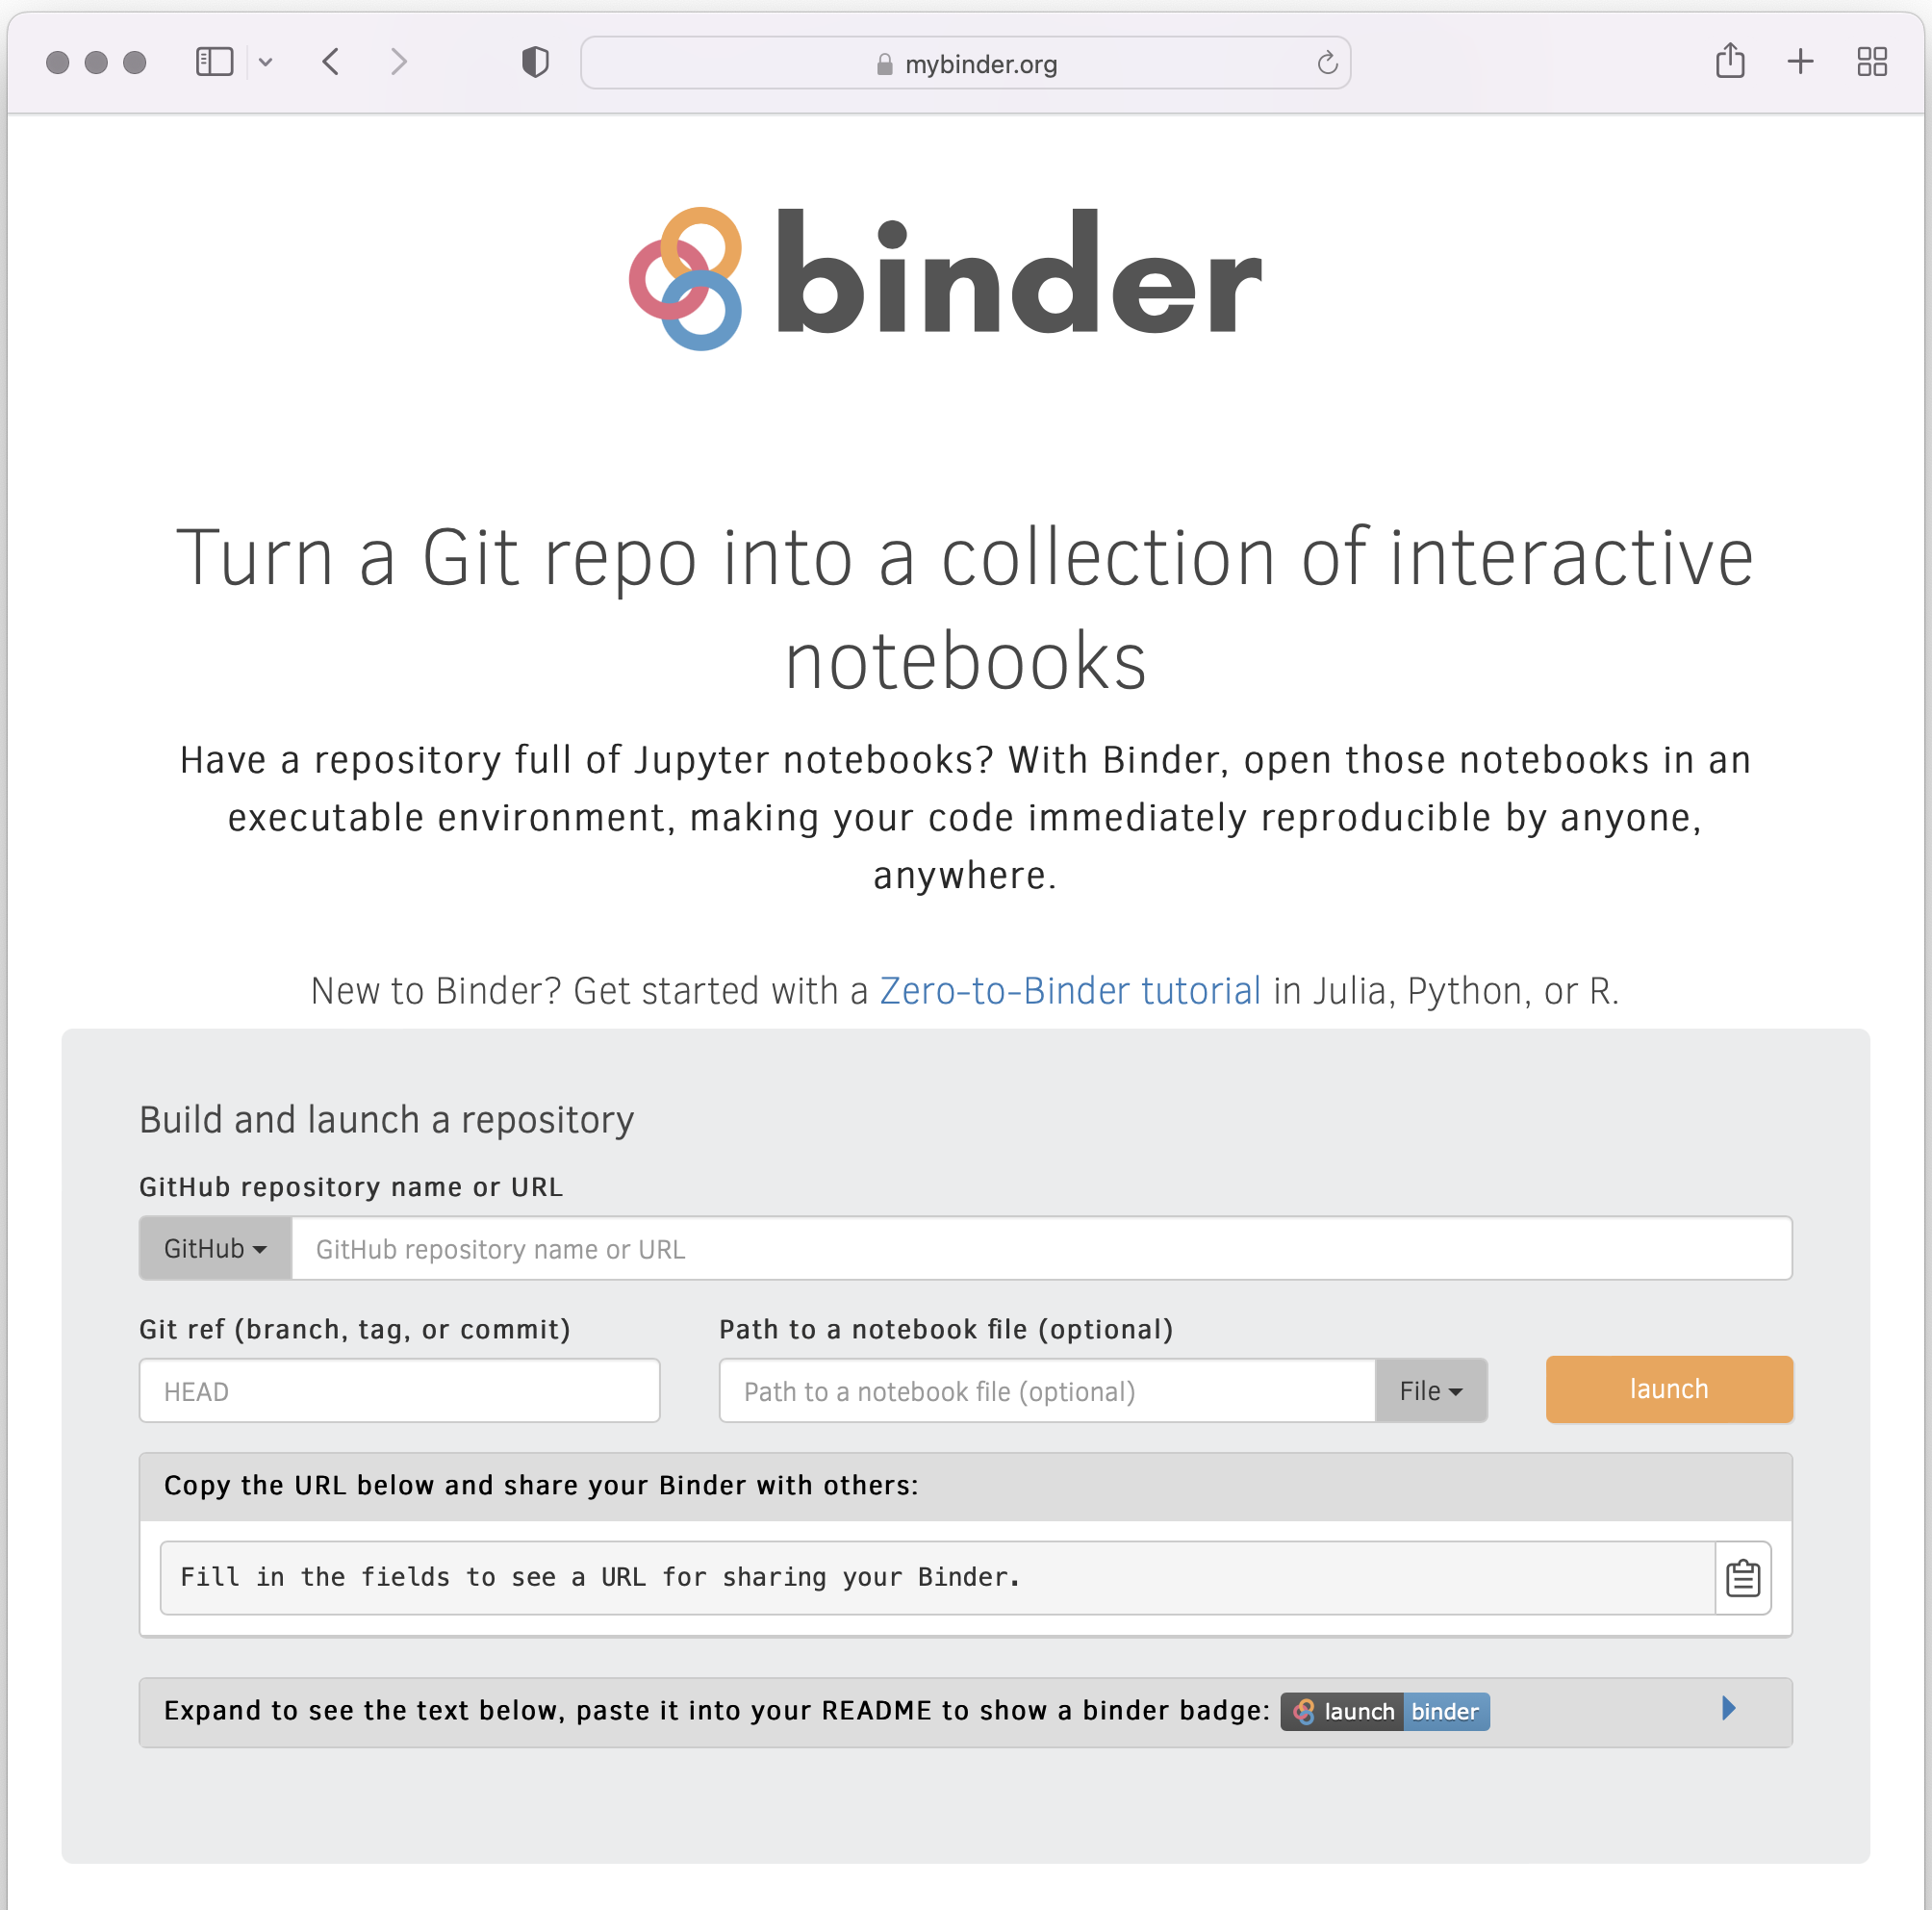
\includegraphics[width=1.0\textwidth]{images/mybinder.png}
  \end{minipage}\hfill
  \begin{minipage}[b]{0.3\textwidth}
    \caption{Home page of the \mybinder{} service.}  \label{fig:mybinder-homepage}
  \end{minipage}
\end{figure}


\begin{compactitem}
\item The \mybinder{} service is called with a URL that encodes the location of the data
  repository\footnote{For example the 
    {\url{https://mybinder.org/v2/gh/fangohr/reproducibility-repository-example/HEAD?labpath=figure1.ipynb}}
    refers to the GitHub repository ``reproducibility-repository-example'' of the
    github user ``fangohr'', asking to open the ``figure1.ipynb'' file.}

  Alternatively, there is form (see Figure~\ref{fig:mybinder-homepage})
  which users can complete with repository details
  to start the build of the corresponding environment, or to obtain the URL to
  re-use that configuration later, or share it with others.
\item From the \mybinder{} entry point, the request is forwarded to one
  \binderhub{} service of one of the organisations in the BinderHub federation
  that has available compute resources.
\item The \binderhub{} software running at the chosen location, will ask
  \repotodocker{} to create a Docker container in which the notebooks from the repository can be executed.
\item \repotodocker{} searches the repository for specifications of software requirements (see \ref{repo2docker-supported-software-specifications}).
\item \repotodocker{} composes a Dockerfile that contains all the commands
  necessary to install software.
\item \repotodocker{} builds the Docker image based on the Dockerfile.
\item \binderhub{} takes the Docker image and asks Kubernetes to start 
  a container based on this image.
\item The notebook server is started in this Docker container.
\item \binderhub{} forwards the user who requested this virtual environment to
  the URL at which the repository (or a particular notebook) can be explored
  from within the Jupyter notebook (which runs in the container).
\end{compactitem}

\paragraph{The repo2docker software tool.}\label{sec:repo2docker}

\repotodocker{} is a tool to fetch a remote repository and build a software
environment for this repository. Currently, \repotodocker{} can retrieve
repositories from the following services and formats: GitHub, Gist, Git, GitLab,
Zenodo, Hydroshare, Figshare, Dataverse.

For the automatic building of reproducible computational environments,
\repotodocker{} understands commonly used conventions for environment specifications and
community standard tools such as Docker, conda, mamba, and pip. See
Section~\ref{repo2docker-supported-software-specifications} below for a full list of
currently supported software specifications.

\paragraph{Supported software specification formats}
\label{repo2docker-supported-software-specifications}
The \repotodocker{} tool currently supports the following software specification
formats to build Docker images:
% source:
% https://repo2docker.readthedocs.io/en/latest/config_files.html#config-files
% 9 April 2022
\begin{compactitem}
\item \softwarename{requirements.txt}, \softwarename{setup.py},
  \softwarename{Pipfile}, \softwarename{Pipfile.lock}: to specify Python
  packages and environments
\item \softwarename{Project.toml}, \softwarename{JuliaProject.toml} and (legacy)
  \softwarename{REQUIRE}: to
  specify Julia version and packages
\item \softwarename{install.R}, \softwarename{DESCRIPTION}: to install R
  libraries, or install the repository as R package
\item \softwarename{apt.get}: to install Debian packages. The Docker container
  is currently based on Ubuntu, which uses the Debian package management tool \softwarename{apt}.
\item \softwarename{environment.yml}: to specify conda or mamba packages and
  environments
\item \softwarename{default.nix}: to use the nix package manager for software provision
\item \softwarename{Dockerfile}: providing a Dockerfile enables users to define
  virtually arbitrary environments, for example based on software from the
  repositories of Linux distributions.
\end{compactitem}

\paragraph{BinderHub}\label{sec:binderhub}
BinderHub is software for hosting a web service built on \repotodocker{} and
JupyterHub where individuals can share reproducible environments for
immediate and free interaction by readers in their browser.


\paragraph{The \mybinder{} service}\label{sec:mybinder}

\emph{\mybinder{}} is a service run by the \emph{BinderHub
  federation}\footnote{\url{https://mybinder.readthedocs.io/en/latest/about/federation.html}}
of organisations. Collectively, they host a service running the BinderHub software
which can be reached from \url{https://mybinder.org}.

The service is actively used with approximately 200,000 sessions being
requested and delivered by the \mybinder{} service every week in 2021. The number
of sessions is growing from approximately 10,000 per day in November 2018
(beginning of the available records) to about 30,000 per day in 2022. We have
identified 60,000 unique repositories published in the last few years which have
used the \mybinder{} service. The data is available~\cite{mybinder-archive}.

Examples of reproducible repositories that make use of the \mybinder service
include reproducible research repositories
\cite{GitHubRepoExampleAlbert2016,Beg2021}, interactive textbooks
\cite{Fangohr2022,Zeller2022} and citizen science and outreach activities
\cite{ligo-open-science,OSCOVIDA2022}.

This \TheProject{} project will not provide or operate a BinderHub service (such as the global
``\url{https://mybinder.org}'' instance). The improvements achieved, however, will immediately
be made available to all operators of BinderHubs, including \mybinder{}.


% \subsubsection{Binder for reproducibility}\label{sec:binder-for-reproducibility}
% \TOWRITE{}{Hmm -- perhaps we don't need this section, as we explain in the
%   Methodology section what we want to do with Binder?}




%%% Local Variables:
%%% mode: latex
%%% TeX-master: "proposal"
%%% End:



% Not relevant here. Should remove that file later.
% % This section is probably not needed for SOURCE.

\medskip
\noindent\textbf{Jupyter as a basis for web services}\\
Because the Jupyter notebook is a web-based application, it can be
deployed at computational facilities or in the cloud, and can function
as the basis for services exposing computational resources of all
kinds to researchers and the public.  Because Jupyter is
\textbf{interactive}, it enables making scientific results and
communications more interactive than static publications.  The
audience can follow their own initiative and ask their own questions
of published data without needing support from the publishing author,
greatly facilitating the \textbf{practicality of Open Science}.

\medskip
\noindent\textbf{Jupyter is generic}\\
\TheProject chose Jupyter because it is
Generic.  Jupyter makes no domain-specific or even language-specific
assumptions.  Any application where mixing description, code, and
results is valuable can make use of Jupyter.  This broad applicability
makes investment in the Jupyter ecosystem extremely effective, because
improvements to Jupyter can serve many communities simultaneously.

Jupyter is built from a collection of standard protocols and file
formats.  Jupyter is not just a single, monolithic piece of
software, but a description of how such software can be built.  The
result is the ability for a variety of communities and applications to
use components of Jupyter for their purposes, and/or reimplement pieces to
meet their needs.
%
For example:
\begin{enumerate}
\item The notebook file format is a well-specified JSON document,
  which can be interpreted by many systems.  This has facilitated the
  development of different services providing rendering of notebooks, e.g. the code
  hosting website GitHub, which renders notebooks for easy viewing by
  anyone, without Jupyter software.
\item The Jupyter protocol describes how execution is performed, which
  has enabled the development of over one hundred kernel
  implementations in dozens of languages\footnote{\url{https://github.com/jupyter/jupyter/wiki/Jupyter-kernels}}.
\item Output in the Jupyter protocol uses web-standard MIME types,
  enabling any possible format to be an output in a Jupyter notebook.
\item The JupyterLab extension system provides a system for building
  applications from Jupyter components and others.
\item The Jupyter Widgets provide a system for customising and
  extending interactivity in Jupyter-based environments.
\end{enumerate}

The popularity of Jupyter, with millions of users and hundreds of open
source contributors, is an indicator of the value and impact of this approach.

\medskip
\noindent\textbf{Improvement to the Jupyter ecosystem}\\
The benefits of focusing our work on a mature system like Jupyter include:

\begin{itemize}
\item vibrant community ensures health and sustainability,
\item large existing user base maximises impact of contributions,
\item mature software ecosystem maintains quality software through
  industry standards such as version control, tests, continuous
  integration, stable release cycles, roadmaps, and user support.
\end{itemize}

The Jupyter community aims to be inclusive, and \TheProject fully
embraces and supports that approach.  Jupyter is inclusive across a number of axes.
By being applicable across numerous domains, Jupyter and \TheProject
encourage participation from individuals of various interests and
backgrounds, and has taken action to improve diversity in the project
by participating in ``Outreachy,'' a program of paid internships for
individuals from groups that face under-representation, systemic bias,
or discrimination.  Jupyter has also operated workshops focused on
training contributors from under-represented groups.  In being free,
public, open source software, Jupyter and \TheProject are accessible
to as many individuals as possible, and invites users and contributors
beyond origin, nationality, beliefs, orientation.  One area where
Jupyter has lacked in this regard is in the User Interface
accessibility, and we will help improve this in
% \taskref{core}{accessibility}
.  Additionally, the project will
focus some of its workshops in
% \taskref{education}{workshops}
on
under-represented communities.


\begin{figure}[ht!]\centering
  \includegraphics[width=0.6\textwidth]{images/notebook_components.png}
  \caption{The architecture of the Jupyter notebook, kernels, and tools
        which operate on notebook files}
  \label{fig:notebook-architecture}
\end{figure}


\subsubsection{Methodology}\label{sec:methodology}

Our approach is centered around the following ideas:
\begin{compactenum}
  \item We put the researcher into the center of our work. In the end,
    researchers need to lead or the very least contribute to make their work
    reproducible. It is thus essential to find technical and social solutions
    that are \emph{useful and practical}. This idea is reflected in researchers
    being involved in \WPref{management} through the \emph{Community Engagegment
    Panel}, the requirements gathering and application of the work carried out
  in \WPref{applications} and the interaction with scientists through our
  outreach and engagement activities in \WPref{education}. All of these inputs
  drive the technical software work done in \WPref{reproducibility} and \WPref{impact}.
\item We also need to consider wishes and constraints from other reproducibility
  stakeholders. These include research councils and funders, publishers, research
  infrastructure providers, and educators. There are also opportunities to use the same
  software environment creation to support outreach and
  citizen-science projects (see~\ref{sec:mybinder}). A set of representatives of
  these domains will be gathered in the Community Engagement Panel, and connect
  us with the relevant communities. A list of confirmed panel members is
  available (see~\taskref{management}{community-engagement-panel}) and will be
  extended if the project is funded.
\item The design idea for \repotodocker{} is to build on existing standards and
  conventions. This means that researchers have already created reproducible
  repositories (if they use those conventions to specify software requirements),
  but we have not developed the tool yet to create the software for that
  repository automatically. Following this design choice means that we do not
  expect researchers to learn something just so that \repotodocker{} can
  understand it.
\item Providing useful training plays a key role in enabling and motivating
  researchers to work reproducible. We will explain the benefits for
  reproducible work, and teach good practice for reproducible science such as
  keeping raw data,  meta data and relevant software, using version control and
  automating analysis steps and workflows.
  We will also showcase tools to support the creation (and use) of reproducible
  research artifacts, including those developed through this project.
\item We will explain the possibility of using Jupyter notebooks to create
  reproducible records of computational science, but also support non-notebook
  driven use cases.
\item The measures we advocate to improve reproducibility in science are
  designed to be embedded into the ongoing research activity to minimise the
  additional burden associated with the publication of results.
\item We believe in an agile approach to effective software engineering to get
  the most useful and fast feedback from the use of those features in a real
  world context.
\item All our outputs will be open source and published with permissive
  licenses.
\end{compactenum}


\medskip
\noindent We implement our approach through 5 Work packages:

%\begin{itemize}
%\item
\WPref{management} deals with the admininstrative~(\taskref{management}{admin})
and technical~(\taskref{management}{project-management}) management of the
project, and the organisation of the Community Engagement
Panel~(\taskref{management}{community-engagement-panel}).
    % \item

    \WPref{reproducibility} will improve the robustness of reproducible
    environments through technical work on \repotodocker{} and BinderHub. In
    particular, we will first create a metric to be able to measure our progress
    (\taskref{reproducibility}{repo2docker-checker}), improve the ability create
    software environments for older repositories
    (\taskref{reproducibility}{repo2docker-timemachine}) and improve the
    performance (\taskref{reproducibility}{performance-optimisation}). We
    explicitly allocate some time in \taskref{reproducibility}{maintenance} for
    maintaining the tools we extend and want to build on. Maintenance is crucial
    to creating reliable, sustainable software, but its cost is often swept
    under the rug in funding applications because of the perceived pressure to
    focus on novelty.
    % \item

    \WPref{impact} will extend the feature set of \repotodocker{} to broaden
    the impact of the project. This
    includes to understand more data sources and software specification patters
    (\taskref{impact}{buildpacks}), to refactor the tool to not depend on a
    Kubernetis installation and support other container formats next to Docker
    (\taskref{impact}{constraints}), to export identified software dependencies
    (\taskref{impact}{extract-dependencies}), to support new use cases and to
    better support use outside the Jupyter ecosystem (\taskref{impact}{patterns}).
    % \item

    \WPref{applications} will test, evaluate and apply the improvements from
    work packages \WPref{reproducibility} and \WPref{impact} in real-world
    reproducibility use cases, such as best practice reproducibility show
    cases~(\taskref{applications}{demos}), use of \repotodocker{} on
    decentralised hardware~(\taskref{applications}{binder-at-home}), publishing
    of large, complex or restricted access data
    sets~(\taskref{applications}{data-publishing}), and reproducibility for HPC~
    (\taskref{applications}{binder-at-hpc}).
    % \item

    \WPref{education} disseminates outcomes, delivers training materials
    and activities, and supports community engagement. We will develop best practice guidelines for reproducible
    science (\taskref{education}{online-resources}), organise and deliver
    training events (\taskref{education}{workshops}), work closely with
    scientists wishing to contribute to the project (\taskref{education}{community-support}).
  %\end{itemize}

% 
% \textbf{Improving the robustness of reproducible environments (\WPref{reproducibility})}\\
% Finally, we are explicitly allocating time in \WPref{reproducibility} for maintaining
% Jupyter software, as well as new development
%  % (\taskref{reproducibility}{maintenance}).
% Maintenance is crucial to creating reliable, sustainable software,
% but its cost is often swept under the rug in funding applications
% because of the perceived pressure to focus on novelty.
% Being up front and explicit about this cost is critical to the sustainability
% of open source open science.
% 
% \medskip
% \noindent\textbf{Broadening  (\WPref{impact})}\\
% In addition to improving how successfully and how often tools like \repotodocker{} reproduce environments,
% we aim to broaden the impact of the tools by making them useful in more contexts.
% The existing software makes certain assumptions about where it will run,
% made for the purposes of limiting maintenance scope of the Binder project.
% As the project has matured, certain expansions of scope are appropriate,
% as seen in the existing demand for new features in the project.
% 
% We further propose improvements to the wider Binder ecosystem
% to expand the impact of the tools in more contexts to be useful to more researchers
% and more institutions.
% In particular, we have identified planned improvements:
% 
% \begin{itemize}
%   \item Binder and its crucial software component \emph{repo2docker}
%   \item relaxing Kubernetes assumption
%   \item running on HPC
%   \item more buildpacks
%     % (\taskref{ecosystem}{r2d-and-binder}).
% 
% \end{itemize}
% 

%   \medskip\noindent\textbf{Beyond the improvement to \TheProject tools
%   (\WPref{applications}, \WPref{education})}\\
% Beyond the improvement to the Binder tools for reproducility, we plan on
% \begin{itemize}
% \item Design, implementation, application, demonstration and
%   evaluation of multiple demonstrators, that cover research fields such as
%   \TOWRITE{}{photon and neutron science, geosciences},
%   and also interests of participating SMEs (\WPref{applications}).
% \item Producing \emph{training and education material} to disseminate
%   the ability to do reproducible computational science using the tools
%   we develop, among others (\WPref{education}).
% \end{itemize}
% 
% \medskip
% \noindent
% \textbf{The science
%   demonstrators}\label{sec:science-demonstrators-in-concept}\\
% 
% We describe the context and challenges for each demonstrator in this
% section. The particular planned activities are shown in the
% corresponding tasks in \WPref{applications}.


\subsubsection{Gender aspects}\label{sec:gender}

\eucommentary{Describe how the gender dimension (i.e. sex and/or gender
  analysis) is taken into account in the project's research and innovation
  content [e.g. 1 page]. If you do not consider such a gender dimension to be
  relevant in your project, please provide a justification.}

\eucommentary{
	Note: This section is mandatory except for topics which have been identified
  in the work programme as not requiring the integration of the gender dimension
  into R\&I content.
}

\eucommentary{
	Remember that that this question relates to the content of the planned
  research and innovation activities, and not to gender balance in the teams in
  charge of carrying out the project.
}

\eucommentary{
	Sex and gender analysis refers to biological characteristics and
  social/cultural factors respectively. For guidance on methods of sex/gender
  analysis and the issues to be taken into account, please refer to
  \url{https://ec.europa.eu/info/news/gendered-innovations-2-2020-nov-24\_en}
}

In order to address gender issues, \TheProject is committed to implement
communication and outreach activities for promoting the role of women in science
and STEM: i) present showcases to demonstrate the results of the project through
the eyes of female Research Software Engineers and researchers; ii)
systematically offer hybrid or online training opportunities to encompass the
lack of mobility of some potential attendees; iii) monitor gender participation
to our training, workshops, and hackathons and track progress. Members of the
consortium are involved in a number of programmes and activities who aim at
upskilling women and diversity and inclusion, for instance The Carpentries and
CodeRefinery training programmes and mentoring programs such as Outreachy or
Open Life Science.

\subsubsection{National and international research or innovation activities}

\eucommentary{Describe any national or international research and innovation
  activities whose results will feed into the project, and how that link will be
  established; [e.g. 1 pages]}
\TOWRITE{}{}

\subsubsection{Interdisciplinarity}

\eucommentary{Explain how expertise and methods from different disciplines will be brought together and integrated in pursuit of your objectives. If you consider that an inter-disciplinary approach is unnecessary in the context of the proposed work, please provide a justification. [e.g. 1/2 page]
}
\TOWRITE{}{}

\subsubsection{Open science practices and implementation}

\TheProject will make use of open source licensed software, packages and libraries, following the \href{https://opensource.org/licenses}{OSI recommendations}. 

All codes in this project will be Open Source and collaboratively developed using GitHub, following best software engineering practice 
such as version control, tests and continuous integration.
Training materials will be collaboratively developed through the \href{https://carpentries-incubator.org/}{Carpentries Incubator} 
using the \href{https://cdh.carpentries.org/}{Carpentries Curriculum Development Handbook}: all Carpentries lessons are licensed under  
the \href{https://creativecommons.org/licenses/by/4.0/legalcode}{Creative Commons Attribution version 4.0 (CC-BY)} and any related software under
the \href{https://opensource.org/licenses/MIT}{MIT license}. 

Use cases and showcases will only make use of data that are openly available.

All publications and/or any research data produced within \TheProject will be published Open Access.


\eucommentary{Describe how appropriate open science practices are implemented as
   an integral part of the proposed methodology. Show how the choice of practices
   and their implementation are adapted to the nature of your work, in a way that
   will increase the chances of the project delivering on its objectives [e.g. 1
   page].
% 
   If you believe that none of these practices are appropriate for your
   project, please provide a justification here.
   }
 
\eucommentary{Open science is an approach based on open cooperative work and systematic
   sharing of knowledge and tools as early and widely as possible in the process.
   Open science practices include early and open sharing of research (for example
   through preregistration, registered reports, pre-prints, or crowd-sourcing);
   research output management; measures to ensure reproducibility of research
   outputs; providing open access to research outputs (such as publications,
   data, software, models, algorithms, and workflows); participation in open
   peer-review; and involving all relevant knowledge actors including citizens,
   civil society and end users in the co-creation of R\&I agendas and contents
   (such as citizen science).}
 
\eucommentary{Please note that this question does not refer to outreach actions that may be
   planned as part of communication, dissemination and exploitation activities.
These aspects should instead be described below under 'Impact'.}

\TOWRITE{}{}

\subsubsection{Research Data Management and management of other outputs}

The Data Management Plan (DMP) will be prepared and regularly updated within WP1. All 
data generated, collected, processed and stored will be made available following the 
relevant standards and regulations. Processing of personal data in relation to training, 
hackathons and/or workshop events will comply with GDPR regulations e.g. data 
anonymization and minimization before sharing. 
Procedures to monitor the real-time effectiveness of our dissemination and 
communication strategies will also be GDPR compliant.
We have no plans to collect or produce PII during the project.


\eucommentary{
Research data management and management of other research outputs: Applicants
generating/collecting data and/or other research outputs (except for
publications) during the project must provide maximum 1 page on how the data/
research outputs will be managed in line with the FAIR principles (Findable,
Accessible, Interoperable, Reusable), addressing the following (the description
should be specific to your project): [1 page]
}

\eucommentary{
Types of data/research outputs (e.g. experimental, observational, images, text,
numerical) and their estimated size; if applicable, combination with, and
provenance of, existing data.
}

\eucommentary{
Findability of data/research outputs: Types of persistent and uniqueidentifiers
(e.g. digital object identifiers) and trusted repositories that will be used.
}

\eucommentary{
Accessibility of data/research outputs: IPR considerations and timeline for open
access (if open access not provided, explain why); provisions for access to
restricted data for verification purposes.
}

\eucommentary{
Interoperability of data/research outputs: Standards, formats and vocabularies
for data and metadata. Reusability of data/research outputs:  Licenses for data
sharing and re-use (e.g. Creative Commons, Open Data Commons); availability of
tools/software/models for data generation. }

\TOWRITE{}{}

\begin{draft}
\section*{Todo list for missing subsections}
\begin{verbatim}
- [ ] 1 page: National or international research or innovation activities
- [ ] 0.5 page: bringing together expertise and methods from different disciplines
- [ ] 0.5 page: social science and humanities - how do we integrate them, or why do we not need them
- [X] 1 page: gender dimension. 
- [ ] 1 page: open science practices and implementation
- [ ] 1 page: research data management and management of other research outputs. (Also FAIR)
\end{verbatim}
\end{draft}

%%% Local Variables:
%%% mode: latex
%%% TeX-master: "proposal"
%%% End:
